
\section{Matemática Discreta}
	\subsection{Lógica Proposicional e Eletrônica Digital}
	\begin{frame}{Lógica e Eletrônica - Tabelas Verdades}
		\begin{itemize}
			\item \textbf{Tabela verdade de uma função boleana:} apresenta \textbf{os valores da função} $ y = f(A, B) $ para \textbf{todas as combinações possíveis} dos valores das variáveis.
		\end{itemize}

		\begin{multicols}{2}
			\begin{figure}[h]
				\centering
				\caption{Exemplo de tabela verdade com 2 entradas}
				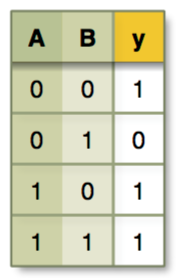
\includegraphics[height=0.35\textheight]{img/ed/ed-tabela_verdade.png}
				\\
				{\footnotesize \textbf{Fonte:} Disponível em: \url{http://eletro.g12.br/arquivos/materiais/eletronica4.pdf}.}
				\label{fig:ed-tabela_verdade}
			\end{figure}
			\columnbreak
			\begin{itemize}
				\item Tabela é \textbf{uma} de várias formas de representação de funções lógicas.
			\end{itemize}
		\end{multicols}
	\end{frame}

	\begin{frame}{Lógica e Eletrônica - Tabelas Verdades}
			\begin{figure}[h]
				\centering
				\caption{Exemplo de tabela verdade com 3 entradas}
				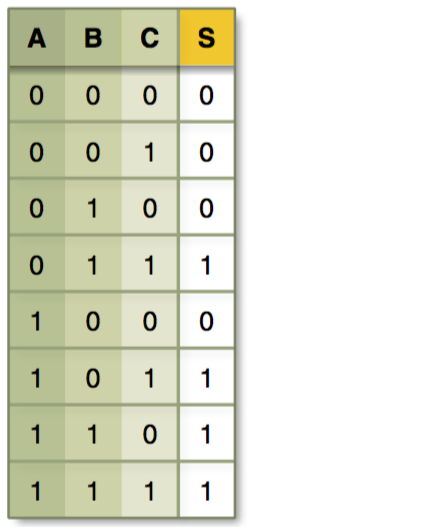
\includegraphics[height=0.7\textheight]{img/ed/ed-tabela_circuito1.png}
				\\
				{\footnotesize \textbf{Fonte:} Disponível em: \url{http://eletro.g12.br/arquivos/materiais/eletronica4.pdf}.}
				\label{fig:ed-tabela_circuito1}
			\end{figure}
	\end{frame}

	\begin{frame}{Lógica e Eletrônica - Tabelas Verdades}
			\begin{figure}[h]
				\centering
				\caption{Exemplo de tabela verdade com 3 entradas }
				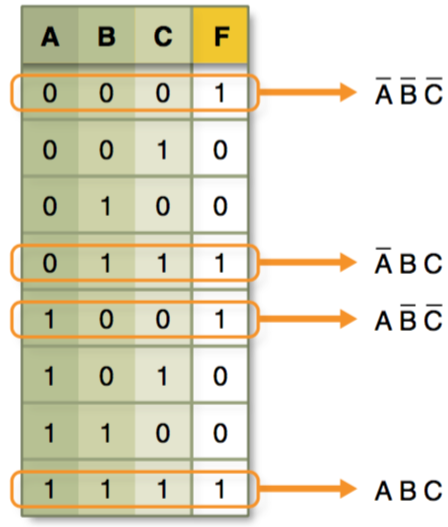
\includegraphics[height=0.7\textheight]{img/ed/ed-tabela_circuito2.png}
				\\
				{\footnotesize \textbf{Fonte:} Disponível em: \url{http://eletro.g12.br/arquivos/materiais/eletronica4.pdf}.}
				\label{fig:ed-tabela_circuito2}
			\end{figure}
	\end{frame}

	\begin{frame}{Lógica e Eletrônica - Portas Lógicas}
		\begin{itemize}
			\setlength\itemsep{1.5em}
			\item \textbf{Portas lógicas:} circuitos eletrônicos básicos que possuem uma ou mais entradas e uma única saída.

			\item Nas entradas e na saída, podemos associar valores booleanos.

				\bigskip

			\item Em eletrônica digital atribuímos valores de tensão
			\begin{itemize}
				\item Associamos ao $ 5 $ V o estado ``$ 1 $'' e ao $ 0 $ V, o estado ``$ 0 $''.
			\end{itemize}
		\end{itemize}
	\end{frame}


	\begin{frame}{Lógica e Eletrônica - Portas Lógicas - Porta NOT}
		\begin{figure}[h]
			\centering
			\caption{Representação da Porta Lógica NOT}
			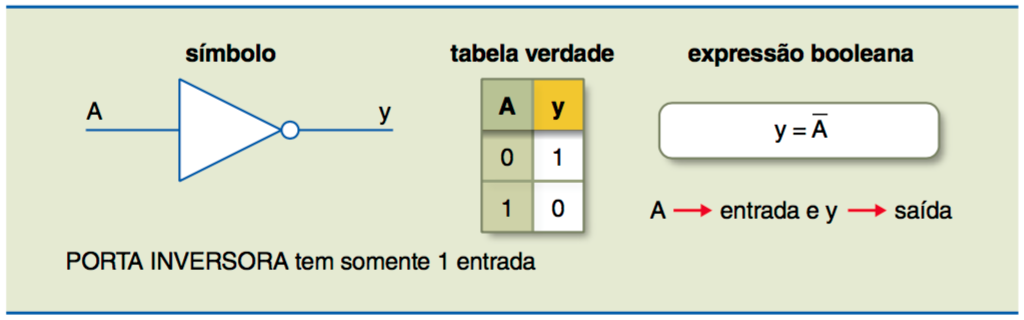
\includegraphics[height=0.55\textheight]{img/ed/ed-porta_not.png}
			\\
			{\footnotesize \textbf{Fonte:} Disponível em: \url{http://eletro.g12.br/arquivos/materiais/eletronica4.pdf}.}
			\label{fig:ed-porta_NOT}
		\end{figure}
	\end{frame}

	\begin{frame}{Lógica e Eletrônica - Portas Lógicas - Porta AND}
		\begin{figure}[h]
			\centering
			\caption{Representação da Porta Lógica AND}
			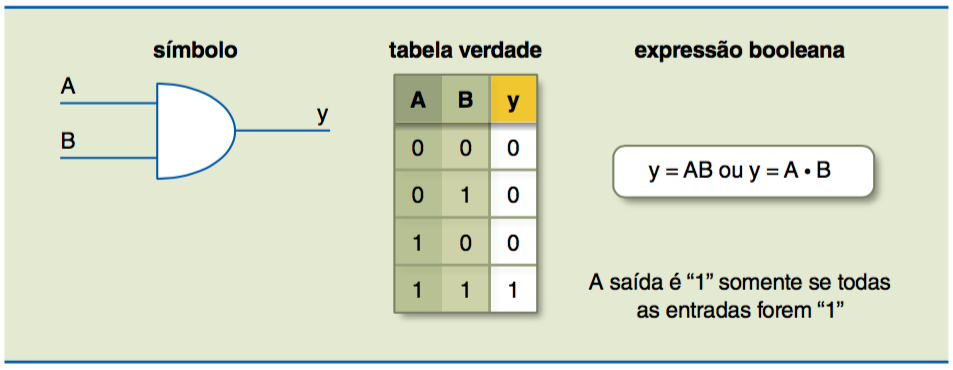
\includegraphics[height=0.66\textheight]{img/ed/ed-porta_and.png}
			\\
			{\footnotesize \textbf{Fonte:} Disponível em: \url{http://eletro.g12.br/arquivos/materiais/eletronica4.pdf}.}
			\label{fig:ed-porta_AND}
		\end{figure}
	\end{frame}

	\begin{frame}{Lógica e Eletrônica - Portas Lógicas - Porta NAND}
		\begin{figure}[h]
			\centering
			\caption{Representação da Porta Lógica NAND}
			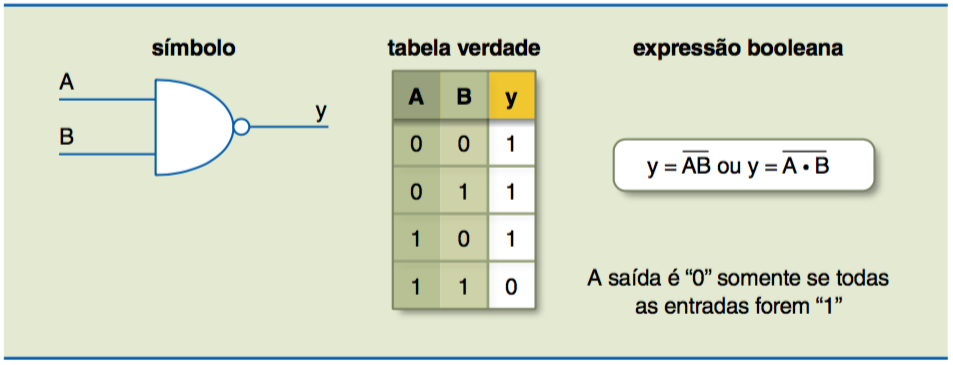
\includegraphics[height=0.66\textheight]{img/ed/ed-porta_nand.png}
			\\
			{\footnotesize \textbf{Fonte:} Disponível em: \url{http://eletro.g12.br/arquivos/materiais/eletronica4.pdf}.}
			\label{fig:ed-porta_NAND}
		\end{figure}
	\end{frame}

	\begin{frame}{Lógica e Eletrônica - Portas Lógicas - Porta OR}
		\begin{figure}[h]
			\centering
			\caption{Representação da Porta Lógica OR}
			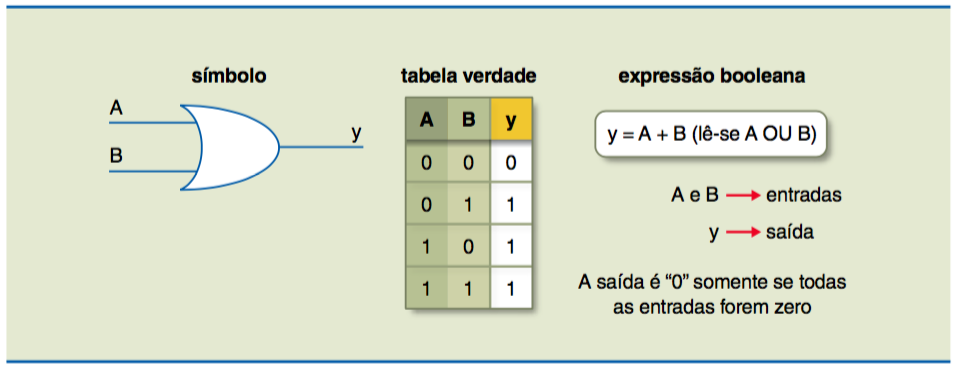
\includegraphics[height=0.66\textheight]{img/ed/ed-porta_or.png}
			\\
			{\footnotesize \textbf{Fonte:} Disponível em: \url{http://eletro.g12.br/arquivos/materiais/eletronica4.pdf}.}
			\label{fig:ed-porta_OR}
		\end{figure}
	\end{frame}

	\begin{frame}{Lógica e Eletrônica - Portas Lógicas - Porta NOR}
		\begin{figure}[h]
			\centering
			\caption{Representação da Porta Lógica NOR}
			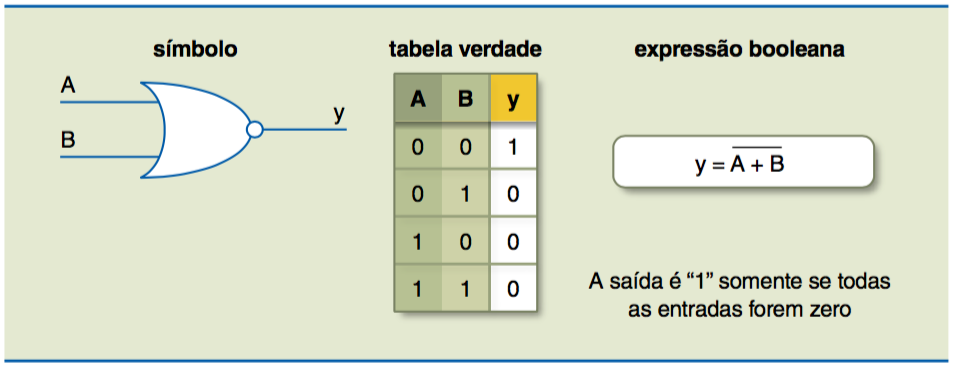
\includegraphics[height=0.66\textheight]{img/ed/ed-porta_nor.png}
			\\
			{\footnotesize \textbf{Fonte:} Disponível em: \url{http://eletro.g12.br/arquivos/materiais/eletronica4.pdf}.}
			\label{fig:ed-porta_NOR}
		\end{figure}
	\end{frame}

	\begin{frame}{Lógica e Eletrônica - Portas Lógicas - Porta XOR}
		\begin{figure}[h]
			\centering
			\caption{Representação da Porta Lógica XOR}
			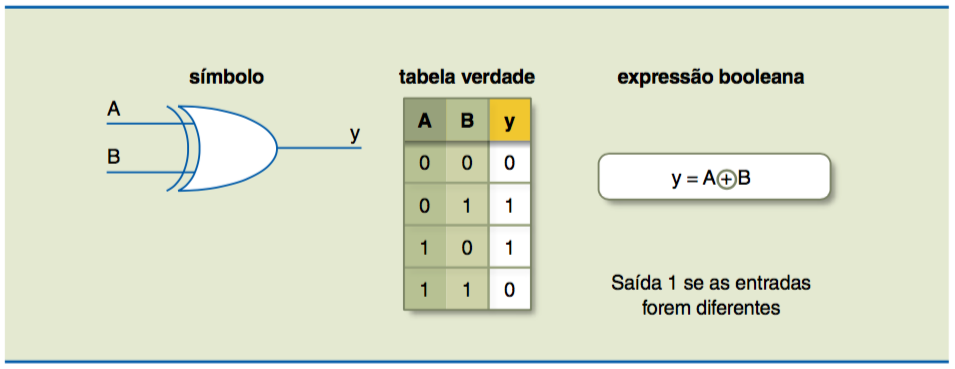
\includegraphics[height=0.66\textheight]{img/ed/ed-porta_xor.png}
			\\
			{\footnotesize \textbf{Fonte:} Disponível em: \url{http://eletro.g12.br/arquivos/materiais/eletronica4.pdf}.}
			\label{fig:ed-porta_XOR}
		\end{figure}
	\end{frame}

	\begin{frame}{Lógica e Eletrônica - Portas Lógicas - Porta XNOR}
		\begin{figure}[h]
			\centering
			\caption{Representação da Porta Lógica XNOR}
			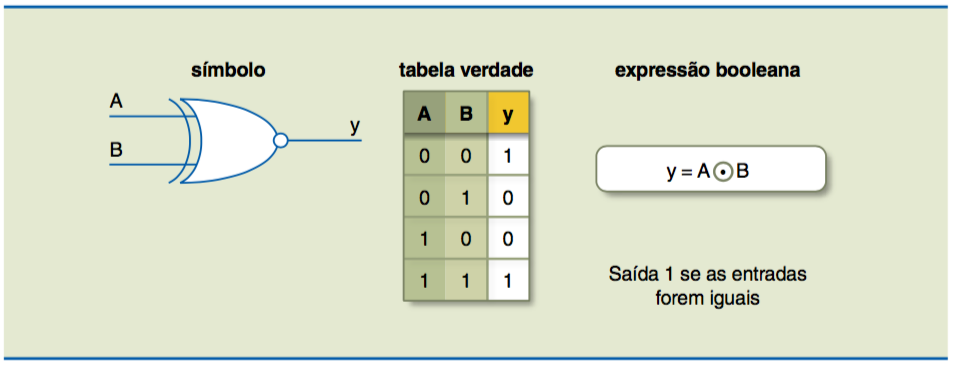
\includegraphics[height=0.66\textheight]{img/ed/ed-porta_xnor.png}
			\\
			{\footnotesize \textbf{Fonte:} Disponível em: \url{http://eletro.g12.br/arquivos/materiais/eletronica4.pdf}.}
			\label{fig:ed-porta_XNOR}
		\end{figure}
	\end{frame}

	\begin{frame}{Lógica e Eletrônica - Circuito Digital}
		\begin{figure}[h]
			\centering
			\caption{Representação de um circuito simples}
			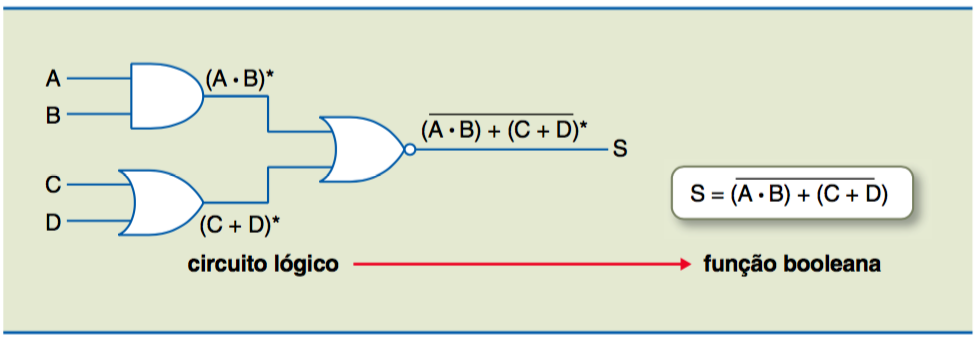
\includegraphics[height=0.6\textheight]{img/ed/ed-circuito.png}
			\\
			{\footnotesize \textbf{Fonte:} Disponível em: \url{http://eletro.g12.br/arquivos/materiais/eletronica4.pdf}.}
			\label{fig:ed-circuito}
		\end{figure}
	\end{frame}
\begin{comment}

	\begin{frame}{Lógica e Eletrônica - Circuito Digital - Circuito Integrado 74147}
		\begin{multicols}{2}
			\begin{figure}[h]
				\centering
				\caption{Circuito Integrado 74147 - codificador com prioridade decimal-BCD}
				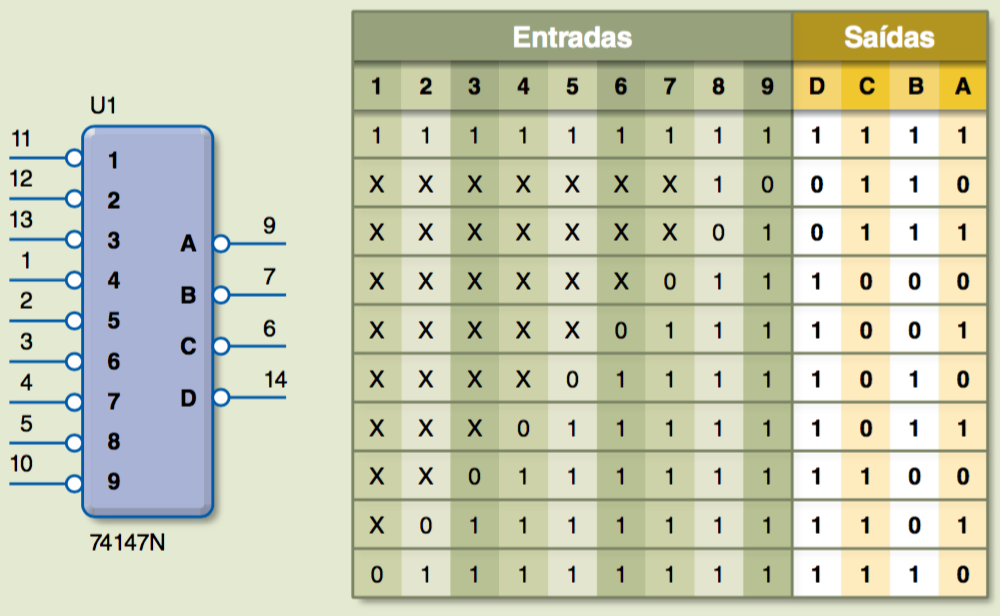
\includegraphics[height=0.6\textheight]{img/ed/ed-74147-tabela.png}
				\\
				{\footnotesize \textbf{Fonte:} Disponível em: \url{http://eletro.g12.br/arquivos/materiais/eletronica4.pdf}.}
				\label{fig:ed-74147-tabela}
			\end{figure}
			\columnbreak
			\pause
			\begin{figure}[h]
				\centering
				%\caption{Exemplo de tabela verdade com 2 entradas}
				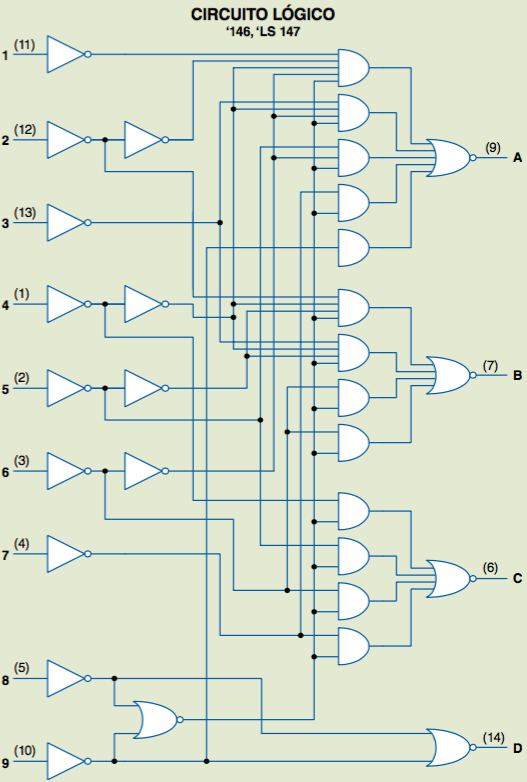
\includegraphics[height=0.93\textheight]{img/ed/ed-74147-circuito.png}
				\label{fig:ed-74147-circuito}
			\end{figure}
		\end{multicols}
	\end{frame}

\end{comment}

	\begin{frame}{Lógica e Eletrônica - Introdução ao Assunto}
		\begin{block}{Questão: Porque falar sobre Portas Lógicas se o assunto da aula é \textit{Hardware} Reconfigurável?}
			\begin{itemize}
				\item Circuitos comprado hoje, como um processador, não permitem que sejam alterados.

				\item E se
			\end{itemize}
		\end{block}
	\end{frame}
